\section{Numerical Results}

We complement the EXIT area identities with exact finite-length calculations
for several CSS code families.  For an erasure probability $e$, let
\[
g_X(e):=\frac{d}{de}\frac{1}{n}\E[H(C_X\mid E,S)]
\]
denote the $X$-component correction-entropy EXIT derivative.  This is one CSS
component of Theorem~\ref{thm:css-exit}.  Its unscaled area is fixed by the
endpoint entropy:
\[
\int_0^1 g_X(e)\,de
=\frac{1}{n}\Bigl(\E[H(C_X\mid E=[n],S)]-\E[H(C_X\mid E=\varnothing,S)]\Bigr)
=\frac{k}{n}.
\]
Thus the numerical area under the unscaled curve is the code rate.  In
Fig.~\ref{fig:scaled-exit-numerics} we instead plot the scaled shape
\[
\widetilde g_X(e):=\frac{g_X(e)}{g_X(1/2)}.
\]
The word ``scaled'' in each legend entry gives the multiplier
$1/g_X(1/2)$ used for visual comparison.

% Three-panel numerical figure for qexit.tex.
% Requires \usepackage{pgfplots} and \pgfplotsset{compat=1.18}.
\begin{figure*}[t]
\centering
\begin{minipage}[t]{0.315\textwidth}
\centering
% Compact PGFPlots panel for the surface5 bit-scale decomposition.
% Requires \usepackage{pgfplots} and \pgfplotsset{compat=1.18}.
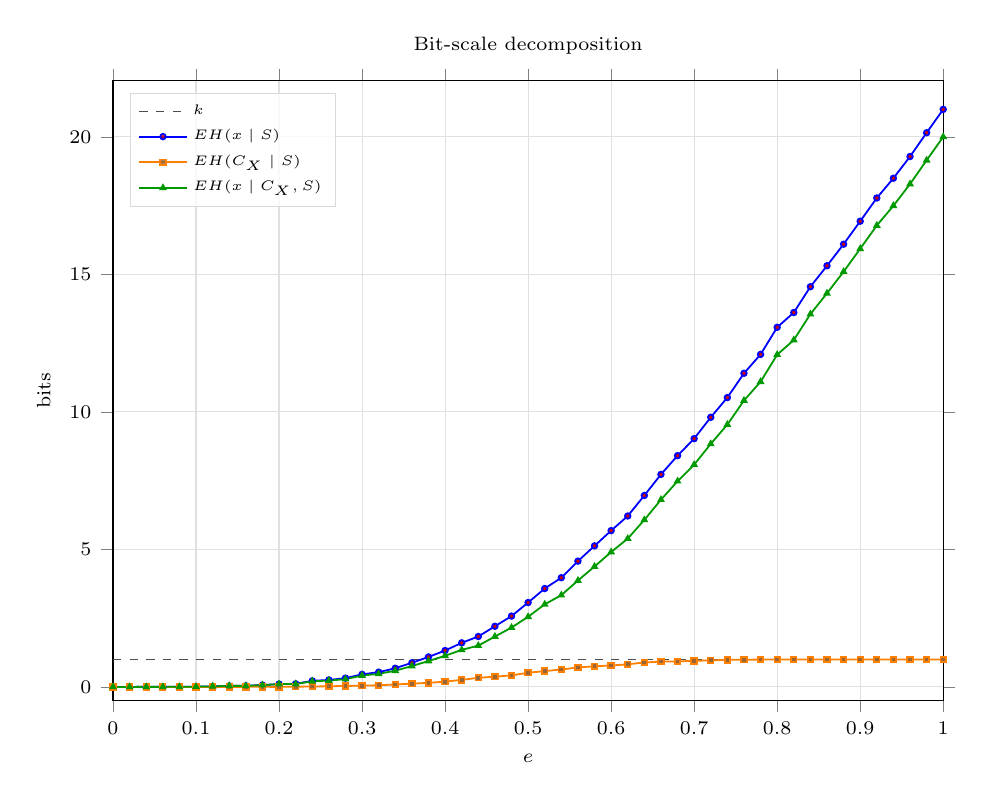
\begin{tikzpicture}
\begin{axis}[
  name=surfaceFiveBitScaleAxis,
  width=\linewidth,
  height=0.78\linewidth,
  title={Bit-scale decomposition},
  title style={font=\scriptsize},
  xlabel={$e$},
  ylabel={bits},
  xmin=0, xmax=1,
  ymin=-0.5, ymax=22.05,
  grid=both,
  major grid style={black!12},
  minor grid style={black!6},
  tick align=outside,
  tick label style={font=\scriptsize},
  label style={font=\scriptsize},
  legend cell align={left},
  legend style={draw=black!15, fill=white, fill opacity=0.82, text opacity=1, at={(0.02,0.98)}, anchor=north west, font=\tiny},
]
\addplot[black!70, dashed, line width=0.55pt] coordinates {(0,1) (1,1)};
\addlegendentry{$k$}
\addplot+[color=blue, mark=*, mark size=1.0pt, line width=0.65pt]
coordinates {(0,0) (0.02,0) (0.04,0.002) (0.06,0.002) (0.08,0.005) (0.1,0.008) (0.12,0.022) (0.14,0.037) (0.16,0.041) (0.18,0.068) (0.2,0.104) (0.22,0.113) (0.24,0.221) (0.26,0.253) (0.28,0.319) (0.3,0.457) (0.32,0.537) (0.34,0.679) (0.36,0.878) (0.38,1.09) (0.4,1.323) (0.42,1.603) (0.44,1.833) (0.46,2.204) (0.48,2.575) (0.5,3.068) (0.52,3.577) (0.54,3.971) (0.56,4.574) (0.58,5.129) (0.6,5.683) (0.62,6.215) (0.64,6.962) (0.66,7.727) (0.68,8.408) (0.7,9.028) (0.72,9.804) (0.74,10.522) (0.76,11.404) (0.78,12.09) (0.8,13.076) (0.82,13.613) (0.84,14.551) (0.86,15.313) (0.88,16.098) (0.9,16.933) (0.92,17.778) (0.94,18.496) (0.96,19.285) (0.98,20.15) (1,21)};
\addlegendentry{$\mathbb{E}H(x\mid S)$}
\addplot+[color=orange, mark=square*, mark size=1.0pt, line width=0.65pt]
coordinates {(0,0) (0.02,0) (0.04,0) (0.06,0) (0.08,0) (0.1,0) (0.12,0.001) (0.14,0) (0.16,0.003) (0.18,0.003) (0.2,0.002) (0.22,0.007) (0.24,0.016) (0.26,0.023) (0.28,0.036) (0.3,0.044) (0.32,0.061) (0.34,0.09) (0.36,0.119) (0.38,0.148) (0.4,0.192) (0.42,0.256) (0.44,0.332) (0.46,0.372) (0.48,0.418) (0.5,0.517) (0.52,0.574) (0.54,0.634) (0.56,0.706) (0.58,0.751) (0.6,0.779) (0.62,0.822) (0.64,0.889) (0.66,0.92) (0.68,0.928) (0.7,0.947) (0.72,0.967) (0.74,0.983) (0.76,0.99) (0.78,0.993) (0.8,0.996) (0.82,1) (0.84,0.997) (0.86,1) (0.88,1) (0.9,1) (0.92,1) (0.94,1) (0.96,1) (0.98,1) (1,1)};
\addlegendentry{$\mathbb{E}H(C_X\mid S)$}
\addplot+[color=green!60!black, mark=triangle*, mark size=1.0pt, line width=0.65pt]
coordinates {(0,0) (0.02,0) (0.04,0.002) (0.06,0.002) (0.08,0.005) (0.1,0.008) (0.12,0.021) (0.14,0.037) (0.16,0.038) (0.18,0.065) (0.2,0.102) (0.22,0.106) (0.24,0.205) (0.26,0.23) (0.28,0.283) (0.3,0.413) (0.32,0.476) (0.34,0.589) (0.36,0.759) (0.38,0.942) (0.4,1.131) (0.42,1.347) (0.44,1.501) (0.46,1.832) (0.48,2.157) (0.5,2.551) (0.52,3.003) (0.54,3.337) (0.56,3.868) (0.58,4.378) (0.6,4.904) (0.62,5.393) (0.64,6.073) (0.66,6.807) (0.68,7.48) (0.7,8.081) (0.72,8.837) (0.74,9.539) (0.76,10.414) (0.78,11.097) (0.8,12.08) (0.82,12.613) (0.84,13.554) (0.86,14.313) (0.88,15.098) (0.9,15.933) (0.92,16.778) (0.94,17.496) (0.96,18.285) (0.98,19.15) (1,20)};
\addlegendentry{$\mathbb{E}H(x\mid C_X,S)$}
\end{axis}
\end{tikzpicture}

{\footnotesize (a) Bit-scale decomposition}
\end{minipage}\hfill
\begin{minipage}[t]{0.315\textwidth}
\centering
\input{fig_scaled_exit_surface_codes_compact.tex}
{\footnotesize (b) Surface-code derivatives}
\end{minipage}\hfill
\begin{minipage}[t]{0.315\textwidth}
\centering
\input{fig_scaled_exit_bivariate_bicycle_codes_compact.tex}
{\footnotesize (c) Bivariate-bicycle derivatives}
\end{minipage}
\caption{Numerical EXIT quantities for CSS codes on the quantum erasure
channel.  Panel (a) shows the bit-scale decomposition for the surface
$[[41,1]]$ code: the raw Pauli ambiguity $\mathbb{E}H(x\mid S)$ decomposes
into correction ambiguity $\mathbb{E}H(C_X\mid S)$ plus the covered-stabilizer
contribution $\mathbb{E}H(x\mid C_X,S)$.  Panels (b) and (c) show scaled
component EXIT derivatives
$\widetilde g_X(e)=g_X(e)/g_X(1/2)$ for surface and bivariate-bicycle code
families.  The scaling shown in each legend is only for visual comparison; the
unscaled area satisfies $\int_0^1 g_X(e)\,de=k/n$.}
\label{fig:scaled-exit-numerics}
\end{figure*}


Panel (a) illustrates the fixed-erasure decomposition behind the CSS EXIT
identity on the $[[41,1]]$ surface code.  The top curve is the raw
$X$-component Pauli ambiguity $\E H(x\mid S)$.  The lower correction curve is
$\E H(C_X\mid S)$, and the gap between them is the covered-stabilizer
contribution $\E H(x\mid C_X,S)$.  Thus the bit-scale plot shows directly the
subtraction of stabilizer degeneracy that converts raw Pauli entropy into
correction entropy.

The surface-code panel uses distances
$d\in\{7,11,21,45,75,251}$.  The unscaled
trapezoidal areas stored for these curves agree with $k/n$ to within
0.006 relative error.  The displayed surface curves are scaled by the
factors listed in the legend, ranging from 20.5
for $d=7$ to $2.07\times 10^{3}$ for
$d=251$.

The bivariate-bicycle panel contains the gross family
$[[576,16]]$ and
$[[2304,16]]$, and the two-gross family
$[[1152,12]]$ and
$[[4608,12]]$.  The corresponding unscaled rates are
0.02778,
0.006944,
0.01042, and
0.002604.  The trapezoidal EXIT areas
match these rates to within 0.0002 relative error over
the sampled window.  Panel (c) repeats the bivariate-bicycle panel as a
placeholder for a third comparison.
